\documentclass[a4paper]{article}

\usepackage[utf8]{inputenc}
\usepackage{enumerate}
\usepackage{amssymb}
\usepackage{amsfonts}
\usepackage{amsthm}
\usepackage{graphicx}
\usepackage[ruled,vlined]{algorithm2e}
\usepackage{color}

%   New commands
\newcommand{\xt}{$(X_t)$}
\newcommand{\om}{$\Omega$ }
\renewcommand\qedsymbol{$\blacksquare$}

%       New Environment

\newtheorem{theorem}{Theorem}
\newtheorem{conjecture}{Conjecture}
\newtheorem{propriete}{Property}[subsection]
\newtheorem{proposition}{Proposition}[subsection]
\newtheorem{corollary}{Corollary}[subsection]
\newtheorem{definition}{Definition}[subsection]
\newtheorem{lemma}{Lemma}[subsection]
\newtheorem{remarque}{Remark}[subsection]

%       Math definitions

\newcommand{\A}{\mathcal{A}}
\newcommand{\p}{\mathcal{P}}
\newcommand{\q}{\mathcal{Q}}
\renewcommand{\S}{\mathcal{S}}
\newcommand{\x}{\mathcal{X}}
\newcommand{\y}{\mathcal{Y}}
\newcommand{\z}{\mathcal{Z}}



%       Line numberwithin
\usepackage[left]{lineno}
\linenumbers


\begin{document}
\section*{Expected results}
Here are the expected results I am willing to present on our paper. Though the list should be exhaustive, I think each of us has something to say on what we should present on the final paper.

\subsection*{Introduction of the ergodic theorem}
The ergodic theorem on Markov Chain requires the irreducibilty and the positive recurrency of the chain, properties we verified on our model. Those properties ensure that our stationnary distribution is unique as well. The ergodic theorem states that for any real-valued function $f$ on our states, its average value (for an enough long walk on our chain) is the same as the expectancy at the stationnary distribution.

\begin{theorem}
  Let $f$ be a real-valued function defined on $\Omega$. If $(X_t)$ is an irreducible and positive recurrent chain, then for any starting distribution $\mu$, we have:
  $$
    \mathbf{P}_\mu \left\{ \lim_{t \rightarrow +\infty} \frac{1}{t} \sum_{s=0}^{t-1} f(X_s) = \sum_{x \in \Omega} f(x)\pi_x \right\} = 1.
  $$
\end{theorem}

In another words, it tells that once we has an large $t$ the mean values of $f(X_t)$ over $t$ is the same as if we has picked a state $x$ at the stationnary distribution $\pi$ and calculate $f$ on it, , here $f$ can be viewed as a propety of a polygon: number of vertices, volume ... Thus it means that we can approach the stationnary distribution by an empirical distribution.

\subsection*{Experimental results list}

For all the following results, the process is the following: run a walk on $(X_t)$ for $k$ in range $[3:100]$ with respectively 1000, 10000, then 100000 steps and compare them with a walk that realises the diameter $\mathcal{D}_{X_t}\leq{2ck^{3/4} + 4(d+1)}$ for $c=1$ and $d=2$. All those results are relevant since it gives us an idea of the distribution on those properties when one reaches the stationnary distribution.

\begin{enumerate}
  \item Number of vertices of a visited polygon: J'ai tout ce qu'il faut, il me reste à lancer les expérimentations.

  \item Largest number of vertices reached in a long run: J'ai les résultats pour 10000, 100000, et le diametre.

  \item Mean volume of polygon: J'ai les résultats pour 1000 et j'aurai assez rapidement le reste.
\end{enumerate}

\begin{figure}
  \begin{center}
    \begin{minipage}[c]{.4\linewidth}
      \resizebox{\columnwidth}{!}{% GNUPLOT: LaTeX picture with Postscript
\begingroup
  \makeatletter
  \providecommand\color[2][]{%
    \GenericError{(gnuplot) \space\space\space\@spaces}{%
      Package color not loaded in conjunction with
      terminal option `colourtext'%
    }{See the gnuplot documentation for explanation.%
    }{Either use 'blacktext' in gnuplot or load the package
      color.sty in LaTeX.}%
    \renewcommand\color[2][]{}%
  }%
  \providecommand\includegraphics[2][]{%
    \GenericError{(gnuplot) \space\space\space\@spaces}{%
      Package graphicx or graphics not loaded%
    }{See the gnuplot documentation for explanation.%
    }{The gnuplot epslatex terminal needs graphicx.sty or graphics.sty.}%
    \renewcommand\includegraphics[2][]{}%
  }%
  \providecommand\rotatebox[2]{#2}%
  \@ifundefined{ifGPcolor}{%
    \newif\ifGPcolor
    \GPcolortrue
  }{}%
  \@ifundefined{ifGPblacktext}{%
    \newif\ifGPblacktext
    \GPblacktextfalse
  }{}%
  % define a \g@addto@macro without @ in the name:
  \let\gplgaddtomacro\g@addto@macro
  % define empty templates for all commands taking text:
  \gdef\gplbacktext{}%
  \gdef\gplfronttext{}%
  \makeatother
  \ifGPblacktext
    % no textcolor at all
    \def\colorrgb#1{}%
    \def\colorgray#1{}%
  \else
    % gray or color?
    \ifGPcolor
      \def\colorrgb#1{\color[rgb]{#1}}%
      \def\colorgray#1{\color[gray]{#1}}%
      \expandafter\def\csname LTw\endcsname{\color{white}}%
      \expandafter\def\csname LTb\endcsname{\color{black}}%
      \expandafter\def\csname LTa\endcsname{\color{black}}%
      \expandafter\def\csname LT0\endcsname{\color[rgb]{1,0,0}}%
      \expandafter\def\csname LT1\endcsname{\color[rgb]{0,1,0}}%
      \expandafter\def\csname LT2\endcsname{\color[rgb]{0,0,1}}%
      \expandafter\def\csname LT3\endcsname{\color[rgb]{1,0,1}}%
      \expandafter\def\csname LT4\endcsname{\color[rgb]{0,1,1}}%
      \expandafter\def\csname LT5\endcsname{\color[rgb]{1,1,0}}%
      \expandafter\def\csname LT6\endcsname{\color[rgb]{0,0,0}}%
      \expandafter\def\csname LT7\endcsname{\color[rgb]{1,0.3,0}}%
      \expandafter\def\csname LT8\endcsname{\color[rgb]{0.5,0.5,0.5}}%
    \else
      % gray
      \def\colorrgb#1{\color{black}}%
      \def\colorgray#1{\color[gray]{#1}}%
      \expandafter\def\csname LTw\endcsname{\color{white}}%
      \expandafter\def\csname LTb\endcsname{\color{black}}%
      \expandafter\def\csname LTa\endcsname{\color{black}}%
      \expandafter\def\csname LT0\endcsname{\color{black}}%
      \expandafter\def\csname LT1\endcsname{\color{black}}%
      \expandafter\def\csname LT2\endcsname{\color{black}}%
      \expandafter\def\csname LT3\endcsname{\color{black}}%
      \expandafter\def\csname LT4\endcsname{\color{black}}%
      \expandafter\def\csname LT5\endcsname{\color{black}}%
      \expandafter\def\csname LT6\endcsname{\color{black}}%
      \expandafter\def\csname LT7\endcsname{\color{black}}%
      \expandafter\def\csname LT8\endcsname{\color{black}}%
    \fi
  \fi
    \setlength{\unitlength}{0.0500bp}%
    \ifx\gptboxheight\undefined%
      \newlength{\gptboxheight}%
      \newlength{\gptboxwidth}%
      \newsavebox{\gptboxtext}%
    \fi%
    \setlength{\fboxrule}{0.5pt}%
    \setlength{\fboxsep}{1pt}%
\begin{picture}(5760.00,5760.00)%
    \gplgaddtomacro\gplbacktext{%
      \csname LTb\endcsname%%
      \put(946,704){\makebox(0,0)[r]{\strut{}$0$}}%
      \put(946,1253){\makebox(0,0)[r]{\strut{}$200$}}%
      \put(946,1803){\makebox(0,0)[r]{\strut{}$400$}}%
      \put(946,2352){\makebox(0,0)[r]{\strut{}$600$}}%
      \put(946,2902){\makebox(0,0)[r]{\strut{}$800$}}%
      \put(946,3451){\makebox(0,0)[r]{\strut{}$1000$}}%
      \put(946,4000){\makebox(0,0)[r]{\strut{}$1200$}}%
      \put(946,4550){\makebox(0,0)[r]{\strut{}$1400$}}%
      \put(946,5099){\makebox(0,0)[r]{\strut{}$1600$}}%
      \put(1387,484){\makebox(0,0){\strut{}$10$}}%
      \put(1829,484){\makebox(0,0){\strut{}$20$}}%
      \put(2271,484){\makebox(0,0){\strut{}$30$}}%
      \put(2712,484){\makebox(0,0){\strut{}$40$}}%
      \put(3154,484){\makebox(0,0){\strut{}$50$}}%
      \put(3596,484){\makebox(0,0){\strut{}$60$}}%
      \put(4038,484){\makebox(0,0){\strut{}$70$}}%
      \put(4479,484){\makebox(0,0){\strut{}$80$}}%
      \put(4921,484){\makebox(0,0){\strut{}$90$}}%
      \put(5363,484){\makebox(0,0){\strut{}$100$}}%
    }%
    \gplgaddtomacro\gplfronttext{%
      \csname LTb\endcsname%%
      \put(198,2901){\rotatebox{-270}{\makebox(0,0){\strut{}volume}}}%
      \put(3220,154){\makebox(0,0){\strut{}$k$}}%
      \put(3220,5429){\makebox(0,0){\strut{}1000 steps run}}%
    }%
    \gplbacktext
    \put(0,0){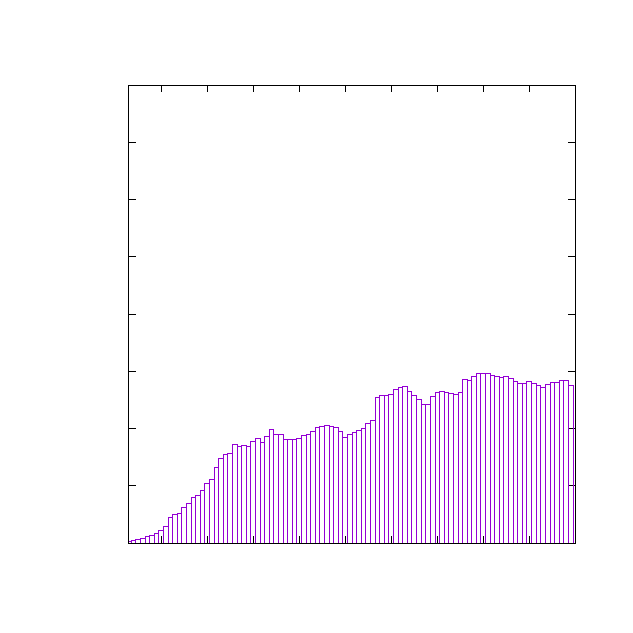
\includegraphics{volume1000}}%
    \gplfronttext
  \end{picture}%
\endgroup
}
    \end{minipage}
    \begin{minipage}[c]{.4\linewidth}
      \resizebox{\columnwidth}{!}{% GNUPLOT: LaTeX picture with Postscript
\begingroup
  \makeatletter
  \providecommand\color[2][]{%
    \GenericError{(gnuplot) \space\space\space\@spaces}{%
      Package color not loaded in conjunction with
      terminal option `colourtext'%
    }{See the gnuplot documentation for explanation.%
    }{Either use 'blacktext' in gnuplot or load the package
      color.sty in LaTeX.}%
    \renewcommand\color[2][]{}%
  }%
  \providecommand\includegraphics[2][]{%
    \GenericError{(gnuplot) \space\space\space\@spaces}{%
      Package graphicx or graphics not loaded%
    }{See the gnuplot documentation for explanation.%
    }{The gnuplot epslatex terminal needs graphicx.sty or graphics.sty.}%
    \renewcommand\includegraphics[2][]{}%
  }%
  \providecommand\rotatebox[2]{#2}%
  \@ifundefined{ifGPcolor}{%
    \newif\ifGPcolor
    \GPcolortrue
  }{}%
  \@ifundefined{ifGPblacktext}{%
    \newif\ifGPblacktext
    \GPblacktextfalse
  }{}%
  % define a \g@addto@macro without @ in the name:
  \let\gplgaddtomacro\g@addto@macro
  % define empty templates for all commands taking text:
  \gdef\gplbacktext{}%
  \gdef\gplfronttext{}%
  \makeatother
  \ifGPblacktext
    % no textcolor at all
    \def\colorrgb#1{}%
    \def\colorgray#1{}%
  \else
    % gray or color?
    \ifGPcolor
      \def\colorrgb#1{\color[rgb]{#1}}%
      \def\colorgray#1{\color[gray]{#1}}%
      \expandafter\def\csname LTw\endcsname{\color{white}}%
      \expandafter\def\csname LTb\endcsname{\color{black}}%
      \expandafter\def\csname LTa\endcsname{\color{black}}%
      \expandafter\def\csname LT0\endcsname{\color[rgb]{1,0,0}}%
      \expandafter\def\csname LT1\endcsname{\color[rgb]{0,1,0}}%
      \expandafter\def\csname LT2\endcsname{\color[rgb]{0,0,1}}%
      \expandafter\def\csname LT3\endcsname{\color[rgb]{1,0,1}}%
      \expandafter\def\csname LT4\endcsname{\color[rgb]{0,1,1}}%
      \expandafter\def\csname LT5\endcsname{\color[rgb]{1,1,0}}%
      \expandafter\def\csname LT6\endcsname{\color[rgb]{0,0,0}}%
      \expandafter\def\csname LT7\endcsname{\color[rgb]{1,0.3,0}}%
      \expandafter\def\csname LT8\endcsname{\color[rgb]{0.5,0.5,0.5}}%
    \else
      % gray
      \def\colorrgb#1{\color{black}}%
      \def\colorgray#1{\color[gray]{#1}}%
      \expandafter\def\csname LTw\endcsname{\color{white}}%
      \expandafter\def\csname LTb\endcsname{\color{black}}%
      \expandafter\def\csname LTa\endcsname{\color{black}}%
      \expandafter\def\csname LT0\endcsname{\color{black}}%
      \expandafter\def\csname LT1\endcsname{\color{black}}%
      \expandafter\def\csname LT2\endcsname{\color{black}}%
      \expandafter\def\csname LT3\endcsname{\color{black}}%
      \expandafter\def\csname LT4\endcsname{\color{black}}%
      \expandafter\def\csname LT5\endcsname{\color{black}}%
      \expandafter\def\csname LT6\endcsname{\color{black}}%
      \expandafter\def\csname LT7\endcsname{\color{black}}%
      \expandafter\def\csname LT8\endcsname{\color{black}}%
    \fi
  \fi
    \setlength{\unitlength}{0.0500bp}%
    \ifx\gptboxheight\undefined%
      \newlength{\gptboxheight}%
      \newlength{\gptboxwidth}%
      \newsavebox{\gptboxtext}%
    \fi%
    \setlength{\fboxrule}{0.5pt}%
    \setlength{\fboxsep}{1pt}%
\begin{picture}(5760.00,5760.00)%
    \gplgaddtomacro\gplbacktext{%
      \csname LTb\endcsname%%
      \put(946,1243){\makebox(0,0)[r]{\strut{}$200$}}%
      \put(946,1793){\makebox(0,0)[r]{\strut{}$400$}}%
      \put(946,2344){\makebox(0,0)[r]{\strut{}$600$}}%
      \put(946,2894){\makebox(0,0)[r]{\strut{}$800$}}%
      \put(946,3445){\makebox(0,0)[r]{\strut{}$1000$}}%
      \put(946,3995){\makebox(0,0)[r]{\strut{}$1200$}}%
      \put(946,4546){\makebox(0,0)[r]{\strut{}$1400$}}%
      \put(946,5097){\makebox(0,0)[r]{\strut{}$1600$}}%
      \put(1387,484){\makebox(0,0){\strut{}$10$}}%
      \put(1829,484){\makebox(0,0){\strut{}$20$}}%
      \put(2271,484){\makebox(0,0){\strut{}$30$}}%
      \put(2712,484){\makebox(0,0){\strut{}$40$}}%
      \put(3154,484){\makebox(0,0){\strut{}$50$}}%
      \put(3596,484){\makebox(0,0){\strut{}$60$}}%
      \put(4038,484){\makebox(0,0){\strut{}$70$}}%
      \put(4479,484){\makebox(0,0){\strut{}$80$}}%
      \put(4921,484){\makebox(0,0){\strut{}$90$}}%
      \put(5363,484){\makebox(0,0){\strut{}$100$}}%
    }%
    \gplgaddtomacro\gplfronttext{%
      \csname LTb\endcsname%%
      \put(198,2901){\rotatebox{-270}{\makebox(0,0){\strut{}volume}}}%
      \put(3220,154){\makebox(0,0){\strut{}$k$}}%
      \put(3220,5429){\makebox(0,0){\strut{}10000 steps run}}%
    }%
    \gplbacktext
    \put(0,0){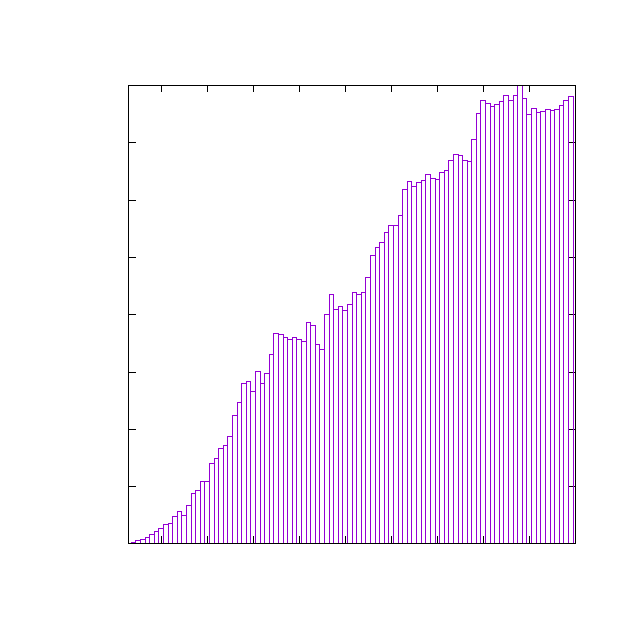
\includegraphics{figure}}%
    \gplfronttext
  \end{picture}%
\endgroup
}
    \end{minipage}
    \caption{Mean volume of a polygon in a long run, $k \in [3-100]$}
    \label{10krun}
  \end{center}
\end{figure}

\subsection*{Theorical result}
Upper bound on the mixing time: this is an important result which gives us an idea on the effectiveness of the sampler.

\end{document}
